\subsection{Test setup}

All benchmarks were performed on a Linux desktop which has 4 GB ram and a Core i3 550 CPU with the following specification:

\begin{itemize}
\item 2 * 3.2 GHz (no Turbo boost)
\item 2 * 32 KB L1 instruction cache
\item 2 * 32 KB L1 data cache
\item 2 * 256 KB L2 cache
\item Shared 4 MB L3 cache
\item 64 byte cache lines
\end{itemize}

Measurements for L1 and L2 cache faults, branch mispredictions and executed instructions were measured with PAPI. For some reason L3 cache faults were unavailable through PAPI. However, we expect the pattern after the cache is exceeded to  to be similar to L1 and L2. Comparison counts were measured with counting integrated into the source code. These counters were removed when running time was measured. The running time was wall time.

% TODO: Type af cache?

All tests were performed 5 times and the median was selected. The data were randomly generated with an uniform distribution. The range of the data was MIN\_INT to MAX\_INT - 1. As mentioned, the max value is MAX\_INT - 1 and not MAX\_INT, because MAX\_INT is used as dummy data. Queries were also randomly generated with the same distribution. Therefore, we were able to make the assumption that the top of the tree is in cache after some number of queries. In contrast, if the queries are sorted then for each query we would have the entire path or almost the entire path in cache. And we would get a linear number of cache faults in total.

% TODO: Noget af ovenstaaende burde nok op da det bruges i vores formeler.

% TODO: Preprocessing er ikke talt med

\subsection{Binary Search}
From the RAM model, we would expect the query time normalized with the
logarithm of the input size, will be a
constant. Figure~\ref{fig:bs_runningtime} clearly shows that this is
not what we experience when running the binary search algorithm on our
test computer.

\begin{figure}[h!]
  \label{fig:bs_runningtime}
  \centering
  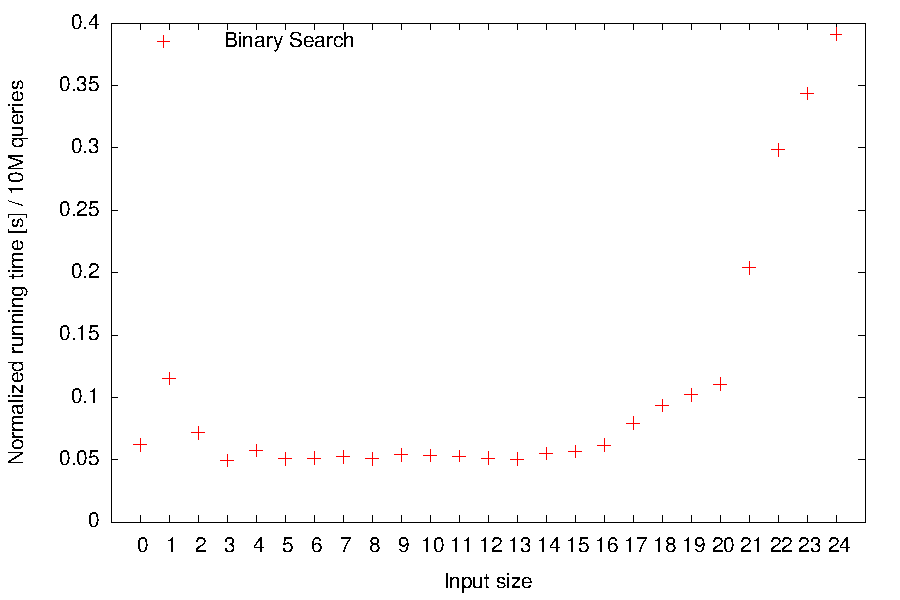
\includegraphics{../week1/plots/outputs/bs_runningtime}
  \caption{Normalized time to perform 10 million queries. The input
    size axis is the base-2 logarithm to the input size.}
\end{figure}

From Figure~\ref{fig:bs_runningtime} we see the first small increase
at input size \(2^{13}\), a somewhat larger increase at \(2^{16}\),
and it behaves very badly after \(2^{20}\).

These numbers corresponds to the CPU's L1, L2 and L3 cache sizes. We
therefore suspect cache faults to be the
bottleneck. Figure~\ref{fig:bs_cachefaults} shows the number of cache
faults per query. It clearly seems that there is a correlation between
where we get cache faults and where the query time gets worse.

\begin{figure}[h!]
  \label{fig:bs_cachefaults}
  \centering
  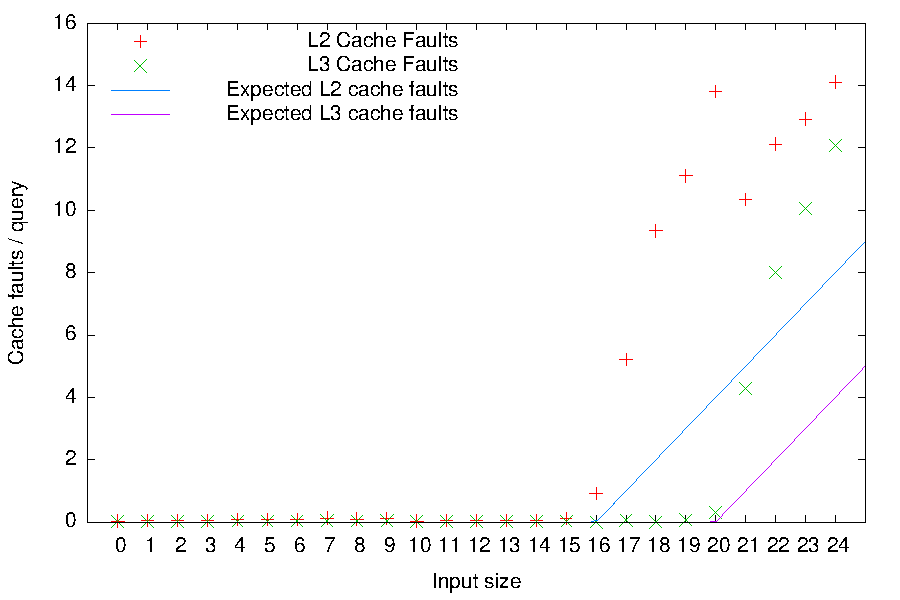
\includegraphics{../week1/plots/outputs/bs_cachefaults}
  \caption{Cache faults measured per query, and the expected number of cache faults.}
\end{figure}

Figure~\ref{fig:bs_cachefaults} shows that we get even more cache
faults than we expect. We think this may be explained by cache
associativity\todo{Should we detail our explanation of this?}.

\subsection{BFS and DFS layout}
In order to improve the query time for large inputs, we will try to
reduce the number of cache faults. We expect a better cache
performance using a BFS or DFS memory
layout. Figure~\ref{fig:bfs_dfs_runningtime} shows the query times of
such layouts.

\begin{figure}[h!]
  \label{fig:bfs_dfs_runningtime}
  \centering
  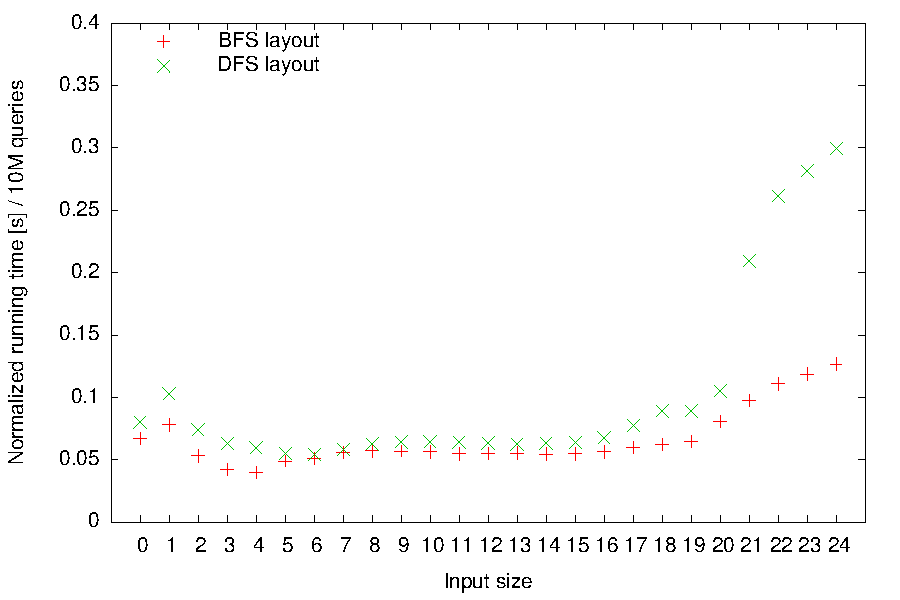
\includegraphics{../week1/plots/outputs/bfs_dfs_runningtime}
  \caption{Normalized query time using BFS/DFS layouts.}
\end{figure}

Both these layouts performs better than the in-order binary search,
but the DFS layout seems to perform worse than the BFS layout.
